\documentclass[11pt]{article}
\usepackage{graphicx} % Required for inserting images
\setlength{\parindent}{0pt}
\usepackage[colorlinks=false,pdfborder={0 0 0},]{hyperref}

\usepackage{enumitem}
\usepackage[utf8]{inputenc}
\usepackage[T1]{fontenc}
\usepackage[english]{babel}
\usepackage{geometry}
\usepackage{lastpage}
\usepackage{fancyhdr}
\usepackage{datetime}

\usepackage[absolute]{textpos}
\usepackage{soul}
\usepackage{tikz}
\usetikzlibrary{calc}

% Link to other SOPs, forms
\usepackage{xr}
\externaldocument[102-]{../2_medical/sop_102_medical}
\externaldocument[302-]{../../300_building/2_fire_gas/sop_302_fire_gas}
% Definitions for SOP sections 3.
\newcommand{\AdverseEvent}{\textbf{Adverse Event}: Any untoward or unfavorable medical occurrence in a human subject, including any abnormal sign, symptom, or disease, temporally associated with the subject's participation in the research, whether or not considered related to the subject's participation in the research.}

\newcommand{\ControlRoom}{\textbf{Control Room}: B17; The main room of the MRI suite that contains the computer displays and keyboards that control the MRI scanner. The Control Room is accessed from B15 that is controlled by an Electronic Lock.}

\newcommand{\DcmComputer}{\textbf{DICOM Computer}: The Mac Studio located in the Control Room the receives DICOM files from the scanner.}

\newcommand{\ElectronicLock}{\textbf{Electronic Lock}: All doors at the ND-HNC are controlled by electronic locks. The electronic lock system recognizes the owner's Irish1Card, logs the time of the attempted entry, and unlocks the door if the owner has been granted access.}

\newcommand{\EEG}{\textbf{EEG}: Electroencephalograpy, a technique used to measure changes in electromagnetic properties of neural tissue.}

\newcommand{\EquipmentRoom}{\textbf{Equipment Room}: B18; The room containing hardware for MRI operations.}

\newcommand{\FDA}{\textbf{FDA}: Food and Drug Administration.}

\newcommand{\GoodCatch}{\textbf{Good Catch}: Early recognition of an event with the potential to cause damage, injury, or illness.}

\newcommand{\Helper}{\textbf{Helper}: Second person in Zones 3 and 4 who assists in emergency responses, typically Level 2-3.}

\newcommand{\Incident}{\textbf{Incident}: An occurence, action, or event that warrants reporting (e.g. a policy is not followed and/or an individual's health is at risk). Includes Adverse Events, Near Misses, Unanticipated Problems, etc.}

\newcommand{\Lead}{\textbf{Lead}: Primary person in Zones 3 and 4 responsible for the Visitor's safety, in charge during emergency responses. Level 4 operator or MRI Technologist.}

\newcommand{\MagnetRoom}{\textbf{Magnet Room}: B17A; The room within the MRI suite that contains the MRI scanner. It is accessed from within the MRI Control room (B17) through a doorway that is controlled by an Electronic Lock.}

\newcommand{\NearMiss}{\textbf{Near Miss}: An incident that occurred but did not cause personal injury/illness e.g. a small/contained fire, trip on sidewalk or carpeting, falling object.}

\newcommand{\NDHNC}{\textbf{ND-HNC}: Notre Dame Human Neuroimaging Center, Lower Level of Veldman Family Psychology Clinic.}

\newcommand{\Operator}{\textbf{Operator}: MRI Technologist or Level 4 researcher, responsible for conducting research operations and maintaining equpiment. The Lead during emergency responses.}

\newcommand{\PIN}{\textbf{PIN}: Personal Identification Number, separate for Irish1Card and security.}

\newcommand{\ResearchAssistant}{\textbf{Research Assistant}: Individual with access Levels 1-3 to the MRI research suite. Typically the Helper during emergency responses.}

\newcommand{\SeriousInjury}{\textbf{Serious Injury}: An injury or illness that is life threatening; results in permanent impairment of a body function or permanent damage to a body structure; or necessitates medical or surgical intervention to preclude permanent damage or impairment.}

\newcommand{\StimControl}{\textbf{Stimulus Control Computer}: The Windows machines in the Control Room that deploy fMRI tasks and capture participant responses.}

% \newcommand{\Subject}{\textbf{Subject}: An individual who is participating in an experimental protocol at ND-HNC and has not taken the ND-HNC safety course.}

\newcommand{\Supervision}{\textbf{Supervision}: A supervisor is continuously present in both sight and sound range of the individual or task being monitored. This approach ensures the supervisor can actively observe, direct, and immediately intervene if a complication or safety issue arises.}

\newcommand{\TMS}{\textbf{TMS}: Transcranial magnetic stimulation, a technique used to disrupt normal operations of neural tissue.}

\newcommand{\TornadoWarn}{\textbf{Tornado Warning}: A tornado has been sighted or indicated by weather radar and there is imminent danger to life and property. Action is required.}

\newcommand{\TornadoWatch}{\textbf{Tornado Watch}: Tornados are possible in and near the watch area. Be ready to act quickly and move to the designated tornado safe area.}

\newcommand{\UnanticipatedProblem}{\textbf{Unanticipated Problem}: An incident, experience, or outcome that meets \textbf{all} of the following criteria: (1) unexpected (in terms of nature, severity, or frequency) given (a) the research procedures that are described in the protocol-related documents, such as the IRB-approved research protocol and informed consent document; and (b) the characteristics of the subject population being studied; (2) related or possibly related to participation in the research; and (3) suggests that the research places subjects or others at a greater risk of harm than was previously known or recognized.}

\newcommand{\VFPC}{\textbf{VFPC}: Veldman Family Psychology Clinic.}

\newcommand{\Visitor}{\textbf{Visitor}: An individual who has not taken the ND-HNC MRI Safety Course but has a legitimate reason for entering the MRI suites. Research participants and their legal guardians are Visitors. Other Visitors may include: individuals providing/receiving a tour of the VFPC and ND-HNC, faculty and staff who have not received MRI Safety Course, and research assistants.}



% figures and tables
\usepackage{graphicx}
\graphicspath{{../../../../media/sops}{../../../../media/nd_brand}}
\usepackage{rotating}
\usepackage{float}
\usepackage{subfig}
\usepackage{caption}
\DeclareCaptionLabelFormat{adja-page}{\hrulefill\\#1 #2 \emph{(previous page)}}

% Branding
\providecommand\fromlogo{nd_logo.png}
\definecolor{NDblue}{RGB}{12,35,64}
\definecolor{NDgold}{RGB}{174,145,66}
\definecolor{NDgray}{RGB}{193,205,221}

% Center info
\providecommand\nameuniversity{University of Notre Dame}
\providecommand\namecenter{Human Neuroimaging Center}
\providecommand\addrcenter{501 N Hill St. South Bend, IN. 46617}
\providecommand\namecollege{College of Arts and Letters}
\providecommand\addrweb{\url{https://neuroimaging.nd.edu}}


% \renewcommand{\headrulewidth}{0pt}
% % \newdateformat{yearmonth}{\THEYEAR-\THEMONTH-\THEDAY}
% \pagestyle{fancy}
% \fancyhead[L]{}
% \fancyhead[R]{Approved: TBD}
% \fancyfoot[C]{}
% \fancyfoot[L]{ND-HNC SOP 101: v.0.4.0}
% \fancyfoot[R]{p. \thepage /\pageref*{LastPage}}

% Format header
\urlstyle{sf}
\pagestyle{fancy}

\fancyhead{}
\fancyhead[L]{%
    % LOGO
    \begin{textblock*}{2in}[0.3066,0.39](1.0in,0.5in)
        \includegraphics[width=2in]{\fromlogo}
    \end{textblock*}

    % Above line
    \begin{textblock*}{6.375in}(1.5in,0.32in)
        \sffamily
        \hfill \textcolor{NDgold} \namecenter\ | \textcolor{NDgold}\namecollege
    \end{textblock*}

    % Below line
    \begin{textblock*}{6.375in}(1.5in,0.53in)
        \sffamily
        \hfill \textcolor{NDgold} \addrcenter\ | \textcolor{NDgold}\addrweb
    \end{textblock*}

    %Line
    \begin{tikzpicture}[remember picture,overlay]
        \draw[color=NDblue,line width=0.7pt] (current page.north west)+(2.45in,-0.48in) -- ($(-0.625in,-0.48in)+(current page.north east)$);
    \end{tikzpicture}
}
\renewcommand{\headrulewidth}{0pt}

% Format footer
\fancyfoot[L]{v.0.4.0}
\fancyfoot[C]{\thepage}
\fancyfoot[R]{\textbf{ND-HNC SOP: 101}}

\renewcommand{\footrulewidth}{0.5pt}


% start document
\begin{document}

\renewcommand{\labelenumii}{\arabic{enumi}.\arabic{enumii}}
\renewcommand{\labelenumiii}{\arabic{enumi}.\arabic{enumii}.\arabic{enumiii}}
\renewcommand{\labelenumiv}{\arabic{enumi}.\arabic{enumii}.\arabic{enumiii}.\arabic{enumiv}}

\begin{center}
	\textbf{\Large SOP 101: Hardware Emergencies}\\
	\hrulefill
\end{center}


\section{Summary}
This document establishes procedures for hardware emergencies at the Notre Dame Human Neuroimaging Center (ND-HNC). They are intended to coordinate a planned response of:

\begin{enumerate}
	\item Moving to safety,
	\item Initiating emergency response,
	\item Coordinating with others in the building,
	\item Protecting responders from the magnetic field, and
	\item Protecting equipment.
\end{enumerate}

For dual responders, the Lead protects the participant and then equipment while the Helper initiates the emergency response.

\section{Scope}
These policies apply to all investigators, research assistants, and ND-HNC staff who enter Zones 3 \& 4 (B15, B17, B17a; Form RO03).

\section{Definitions}

\begin{itemize}
	\item \ControlRoom
	\item \ElectronicLock
	\item \EquipmentRoom
	\item \Helper
	\item \Lead
	\item \MagnetRoom
	\item \Visitor
\end{itemize}

\section{Notes}

\begin{enumerate}
	\item Emergency response and maintenance personnel \textbf{CANNOT} enter the Magnet Room unless they have been screened and all metal objects have been removed.
	\item Emergency response personnel can \textbf{ONLY} enter Zone 3 without completing an MRI Safety screener if the door to the Magnet Room has been locked by key.
	\item Fire extinguishers in the MRI suite are \textbf{NOT} MRI compatible, and cannot be brought into the Magnet Room.
\end{enumerate}

\section{Policies \& Procedures}

In the sections below, several scenarios are depicted regarding hardware emergencies.


% Gas
\subsection{Gas: the Magnet Room is filling with gas and/or vapor.}
\label{ssec:gas}

A magnet quench results in the rapid boil-off of cryogens that maintain the superconductivity of the main field coils. Once in progress a quench cannot be stopped, do not attempt any interventions and stay out of the Magnet Room. While the resulting gases are engineered to exhaust safely through ceiling-mounted vent pipes, a venting system failure will cause these gases to accumulate in the room. Although the cryogens are non-toxic and non-explosive, they present a critical safety risk by displacing oxygen, creating a severe danger of fatal asphyxiation.

\subsubsection*{\textit{Single Responder}}

\begin{enumerate}
	\item If a Visitor is in the scanner, remove them immediately. If the Visitor is injured, follow injury procedures (SOP 102.\ref{102-ssec:injury-cons} or SOP 102.\ref{102-ssec:injury-uncons}).
	\begin{enumerate}
		\item Stay low to the floor below the gas. The room will be cold, water vapor may make visibility in the room poor. A change in pressure may make it difficult to open the Magnet Room door.
	\end{enumerate}
	\item Close and lock the Magnet Room door.
	\item Follow SOP 302.\ref{302-ssec:fire-evac} `Fire or Gas Leak' procedures:
	\begin{enumerate}
		\item Pull the nearest fire alarm (Fig. \ref{fig:vfpc-floor0}).
		\item Gather in the designated Safe Meeting Spot: Northwest corner of parking lot (Fig. \ref{fig:vfpc-rend}).
		\item Call 911 to notify the South Bend Fire Department (SBFD) and say: ``We have gas in the MRI Center at Veldman Family Psychology Clinic, 501 North Hill Street''.
		\item If you are unable to evacuate, draw attention by yelling out.
	\end{enumerate}
	\item Call any MRI staff; MRI staff call Richard Vega (Siemens Engineer).
	\item Prepare to receive and escort SBFD.
	\item Record issue in ND-HNC Form LG01: Hardware Issues.
\end{enumerate}

\subsubsection*{\textit{Dual Responders}}

\begin{enumerate}
	\item Lead
	\begin{enumerate}
		\item If a Visitor is in the scanner, remove them immediately. If the Visitor is injured, follow injury procedures (SOP 102.\ref{102-ssec:injury-cons} or SOP 102.\ref{102-ssec:injury-uncons}).
		\item Close and lock the Magnet Room door.
		\item Proceed to the designated Safe Meeting Spot: Northwest corner of parking lot (Fig. \ref{fig:vfpc-rend}).
		\item Call any MRI staff; MRI staff call Richard Vega (Siemens Engineer).
		\item Prepare to receive and escort SBFD.
		\item Record issue in ND-HNC Form LG01: Hardware Issues.
	\end{enumerate}

	\item Helper
	\begin{enumerate}
		\item If a Visitor is in the scanner, assist with their removal.
		\item Pull the nearest fire alarm (Fig. \ref{fig:vfpc-floor0}).
		\item Gather in the designated Safe Meeting Spot: Northwest corner of parking lot (Fig. \ref{fig:vfpc-rend}).
		\item Call 911 to notify the South Bend Fire Department (SBFD) and say ``We have a possible gas leak in the MRI Center at Veldman Family Psychology Clinic, 501 North Hill Street''.
		\item Assist in receiving, escorting SBFD.
	\end{enumerate}
\end{enumerate}


% Fire
\subsection{Fire or Smoke: present in Magnet or Control Room.}
\label{ssec:fire}

Electrical disruption may spark combustible materials, resulting in fire or smoking. The Magnet Room is equipped with a built-in fire suppression system which should trigger automatically, and both the Magnet Room and Control Room are equipped with fire detectors.

\subsubsection*{\textit{Single Responder}}

\begin{enumerate}
	\item Press the Emergency Power Off (EPO) button (Fig. \ref{fig:button-wall-mag}, C; Fig. \ref{fig:button-wall-con}, C).
	\item If a Visitor is in the scanner, remove them immediately. If the Visitor is injured, follow injury procedures (SOP 102.5.\ref{102-ssec:injury-cons} or SOP 102.5.\ref{102-ssec:injury-uncons}).
	\item Close and lock the Magnet Room door.
	\item \textbf{Fire in Magnet Room}: Do not fight.
	\item \textbf{Fire in Control or Equipment Room}: If possible, use the fire extinguisher in B15 to extinguish the fire (Fig. \ref{fig:fire-ext}).
	\item Initiate Fire Evacuation (SOP 302.\ref{302-ssec:fire-evac}): pull fire alarm (Fig. \ref{fig:fire-alarm}) and evacuate building.
	\item Call 911 to notify the South Bend Fire Department (SBFD) and say: ``We have [fire, smoke] in the MRI Center at Veldman Family Psychology Clinic, 501 North Hill Street''.
	\item Call any MRI staff; MRI staff call Richard Vega (Siemens Engineer).
	\item Prepare to receive and escort SBFD.
	\item Record issue in ND-HNC Form LG01: Hardware Issues.
\end{enumerate}

\subsubsection*{\textit{Dual Responders}}

\begin{enumerate}
	\item Lead
	\begin{enumerate}
		\item Press the Emergency Power Off (EPO) button (Fig. \ref{fig:button-wall-mag}, C; Fig. \ref{fig:button-wall-con}, C).
		\item If a Visitor is in the scanner, remove them immediately. If the Visitor is injured, follow injury procedures (SOP 102.5.\ref{102-ssec:injury-cons} or SOP 102.5.\ref{102-ssec:injury-uncons}).
		\item Close and lock the Magnet Room door.
		\item Call any MRI staff; MRI staff call Richard Vega (Siemens Engineer).
		\item Prepare to receive and escort SBFD.
		\item Record issue in ND-HNC Form LG01: Hardware Issues.
	\end{enumerate}

	\item Helper
	\begin{enumerate}
		\item Initiate Fire Evacuation (SOP 302.\ref{302-ssec:fire-evac}): pull fire alarm (Fig. \ref{fig:fire-alarm}) and evacuate building.
		\item \textbf{Fire in Magnet Room}: Do not fight.
		\item \textbf{Fire in Control or Equipment Room}: If possible, use the fire extinguisher in B15 to extinguish the fire (Fig. \ref{fig:fire-ext}).
		\item Call 911 to notify the South Bend Fire Department (SBFD) and say: ``We have [fire, smoke] in the MRI Center at Veldman Family Psychology Clinic, 501 North Hill Street''.
		\item Assist in receiving, escorting SBFD.
	\end{enumerate}
\end{enumerate}


% Water
\subsection{Water: present in Magnet or Control Room.}
\label{ssec:water}

Plumbing failure or severe storms may result in flooding and electrical disruption.

\begin{enumerate}
	\item Press the Emergency Power Off (EPO) button (Fig. \ref{fig:button-wall-mag}, C; Fig. \ref{fig:button-wall-con}, C).
	\item If a Visitor is in the scanner, remove them immediately. If the Visitor is injured, follow injury procedures (SOP 102.\ref{102-ssec:injury-cons} or SOP 102.\ref{102-ssec:injury-uncons}).
	\item Close and lock the Magnet Room door.
	\item Move to Zone 2.
	\item Call Utilities \& Maintenance (after hours: Notre Dame Police) and say: ``We have flooding in the MRI Center at Veldman Family Psychology Clinic, 501 North Hill Street''.
	\item Call Veldman Reception and say ``We have flooding in the MRI Suite and have called Utilities \& Maintenance.''
	\item Call any MRI staff; MRI staff call Richard Vega (Siemens Engineer).
	\item Prepare to receive and escort Maintenance or Police.
	\item Record issue in ND-HNC Form LG01: Hardware Issues.
\end{enumerate}


% Oxygen
\subsection{O2 Sensor: Alarm sounds.}
\label{ssec:oxygen}

A magnetic quench or smoke in the Magnet Room may trigger the oxygen sensor (Fig \ref{fig:button-wall-mag}, B; Fig. \ref{fig:oxygen}).

\begin{enumerate}
	\item Follow the relevant Gas (SOP 101.\ref{ssec:gas}) or Fire, Smoke (SOP 101.\ref{ssec:fire}) protocol.
\end{enumerate}


% Metal no Visitor
\subsection{Metal: an object is attracted to the magnet, a Visitor is NOT in the bore.}
\label{ssec:metal-no-subj}

Any ferrous material introduced into the Magnet Room will become attracted to the bore. Objects may range in size from the very small (metallic shavings, paper clips) to the intermediate (tools, watch, phone) and the large (chair, fire extinguisher). The very small items will disrupt signal, compromising data quality, while the larger items pose a risk to the magnet itself.

\begin{enumerate}
	\item Do not attempt to remove the object.
	\item Call any MRI staff; MRI staff call Richard Vega (Siemens Engineer).
	\item Record issue in ND-HNC Form LG01: Hardware Issues.
	\item Record compliance issue in ND-HNC Form LG04: Compliance.
\end{enumerate}


% Metal unaffected Visitor
\subsection{Metal: an object is attracted to the magnet, an UNAFFECTED Visitor is in the bore.}
\label{ssec:metal-un-subj}

When a research assistant or MRI personnel enter the Magnet Room during the course of research, perhaps to calibrate the eye tracker or reattach psychophysiologic recording devices, there is a risk that they will introduce a ferrous object into the field.

\begin{enumerate}
	\item Remove the Visitor from the Magnet Room.
	\item Follow procedures in SOP 101.\ref{ssec:metal-no-subj}.
\end{enumerate}


% Pump
\subsection{Pump: you do not hear coolant circulating, or UPS alarms.}
\label{ssec:pump}

The liquid helium of the magnet is kept cool by circulating cryogens, and the pumping system for these cryogens can be heard in rooms B15, B17a, and B18. If the pumps are inoperative for a long enough period, the magnet may lose superconductivity and quench.\\

For short-term power disruption, the pumps are connected to a Universal Power Supply (UPS) which provide a reserve of power and sound an alarm that they have activated. Longer-term power disruption ($>$4 hours) requires a transfer of power from the building (and UPS) to the backup generator.

\begin{enumerate}

	\item To transfer power from building supply to the generator:
	\begin{enumerate}
		\item Navigate to MRI Equipment room (B18).
		\item Identify pump power switch (Fig. \ref{fig:power-switch}).
		\item Avert eyes, move switch from Normal ON to OFF. Wait a moment.
		\item Move switch from OFF to GENERATOR.
	\end{enumerate}
	\item Call any MRI staff. MRI staff call:
	\begin{enumerate}
		\item Christine Schmidt (Haskris); Haskris monitors the cooling system and should contact MRI staff for any issues.
		\item Richard Vega (Siemens Engineer).
	\end{enumerate}
	\item Record issue in ND-HNC Form LG01: Hardware Issues.
\end{enumerate}


% Lock out
\subsection{Access: you are locked out of the Control or Magnet Room.}
\label{ssec:access}

The Control Room door is controlled by an Electronic Lock and will not open unless an authorized Irish1Card is presented. The Magnet Room door is electronically sealed. In the case of power failure, a key can open each door.

\begin{enumerate}
	\item Door to Magnet Room (B17a) does not release: press the emergency release button (Figs. \ref{fig:button-wall-con}, D); twist button clockwise to reset lock.
	\item Door to Control Room (B17) does not open: ensure you have proper access by contacting Allison Collins (Building Management).
	\item Record issue in ND-HNC Form LG01: Hardware Issues.
\end{enumerate}


\section{Figures}

% EPO Pic, magnet
\begin{figure}[H]
	\centering
	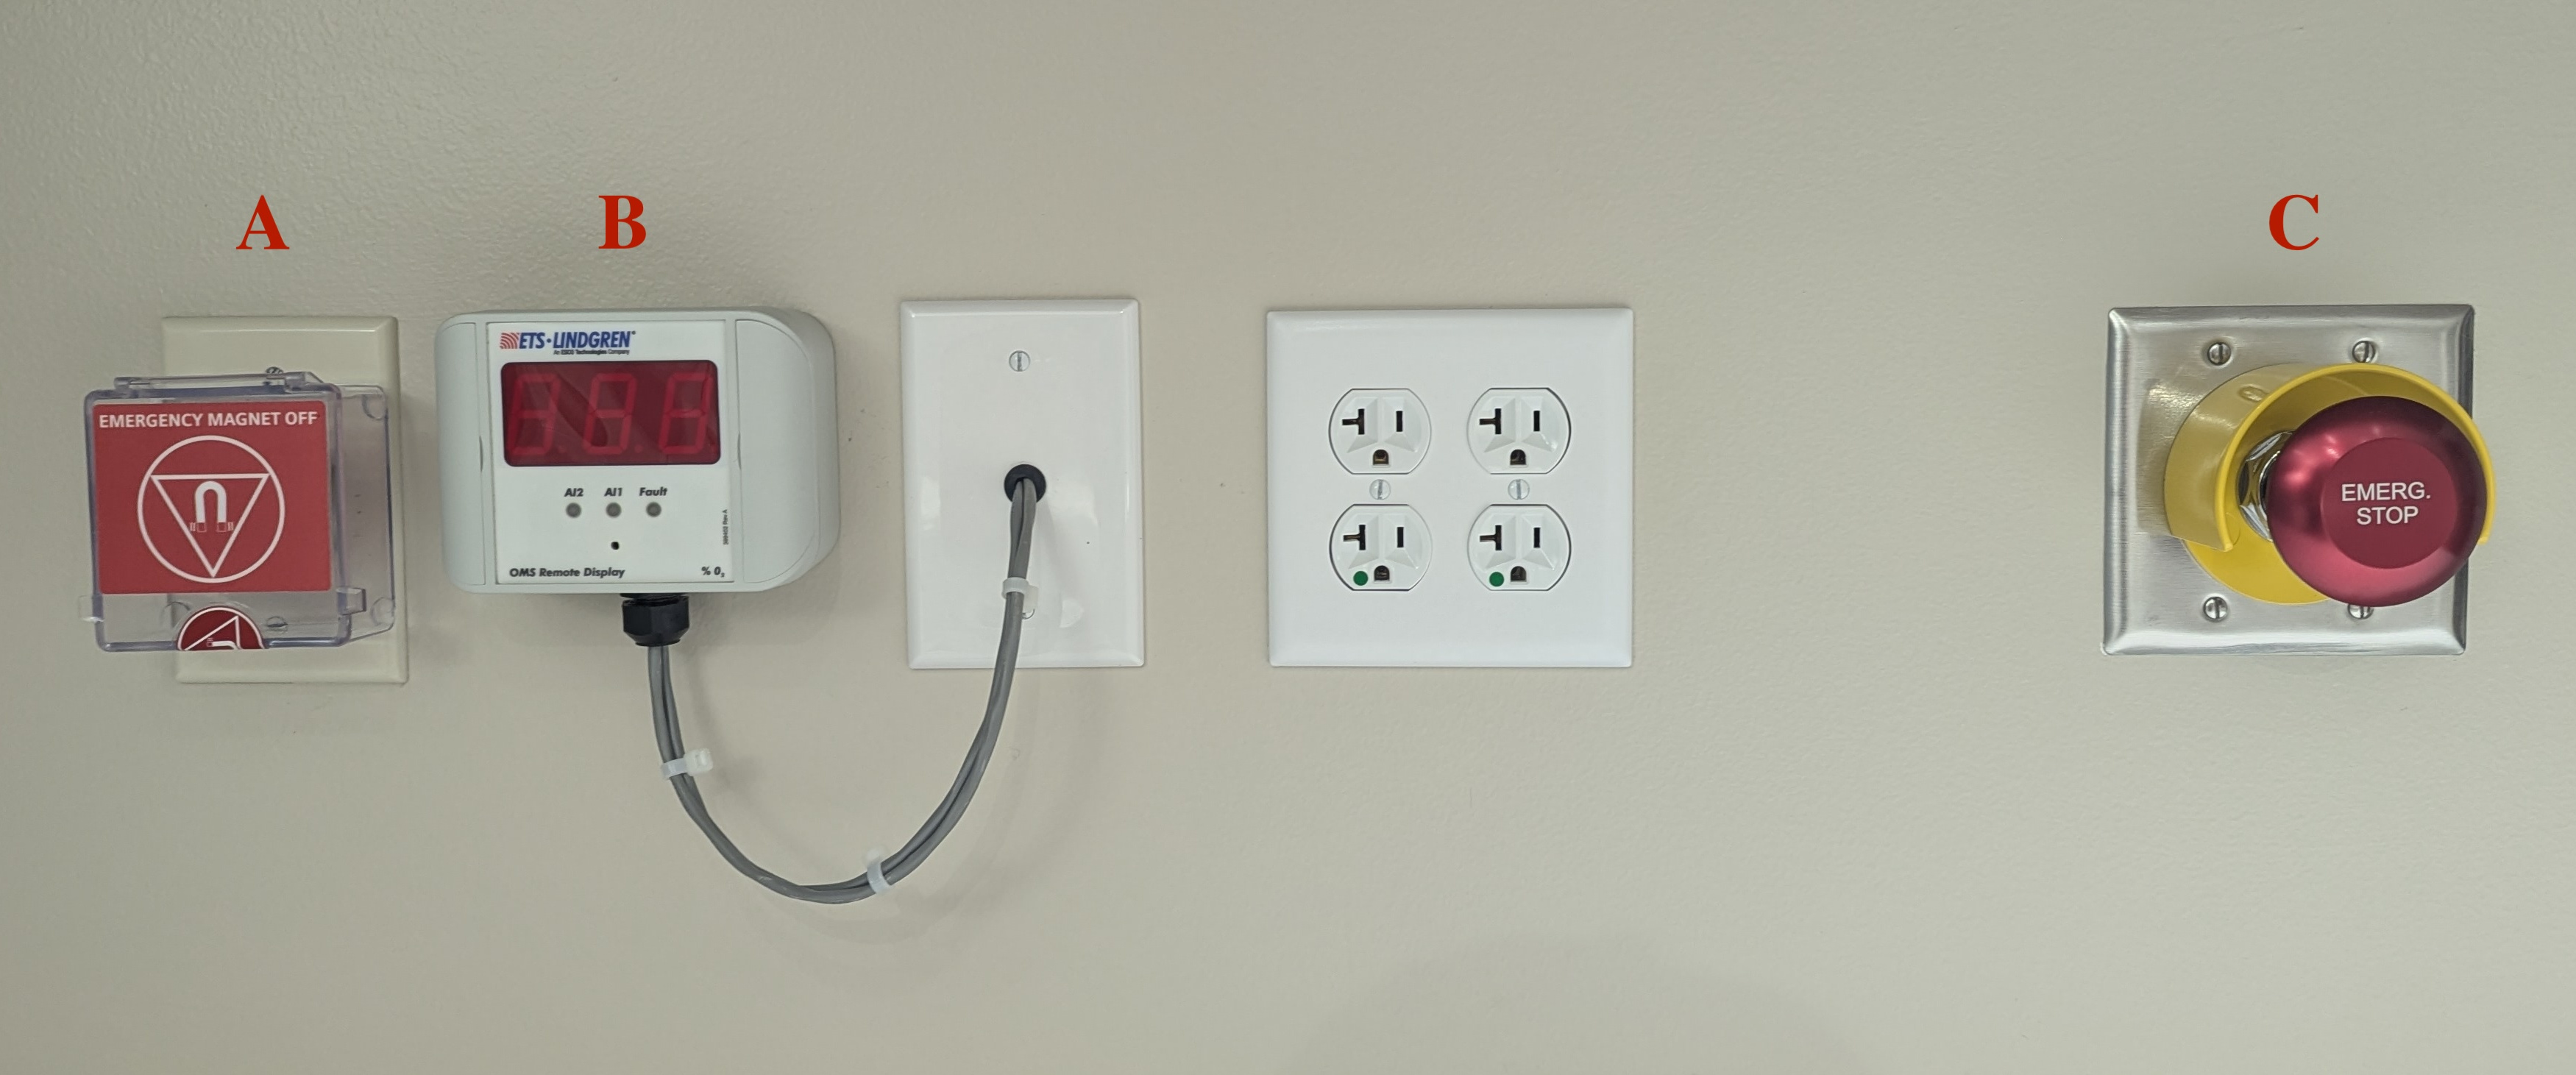
\includegraphics[width=0.95\textwidth]{quench_epo_magnet2.jpg}
	\caption{Magnet Room button wall. \textbf{A} Quench. \textbf{B} Oxygen sensor, alarm. \textbf{C} Emergency Power Off.}
	\label{fig:button-wall-mag}
\end{figure}

% EPO Pic, Control
% TODO: determine E
\begin{figure}[H]
	\centering
	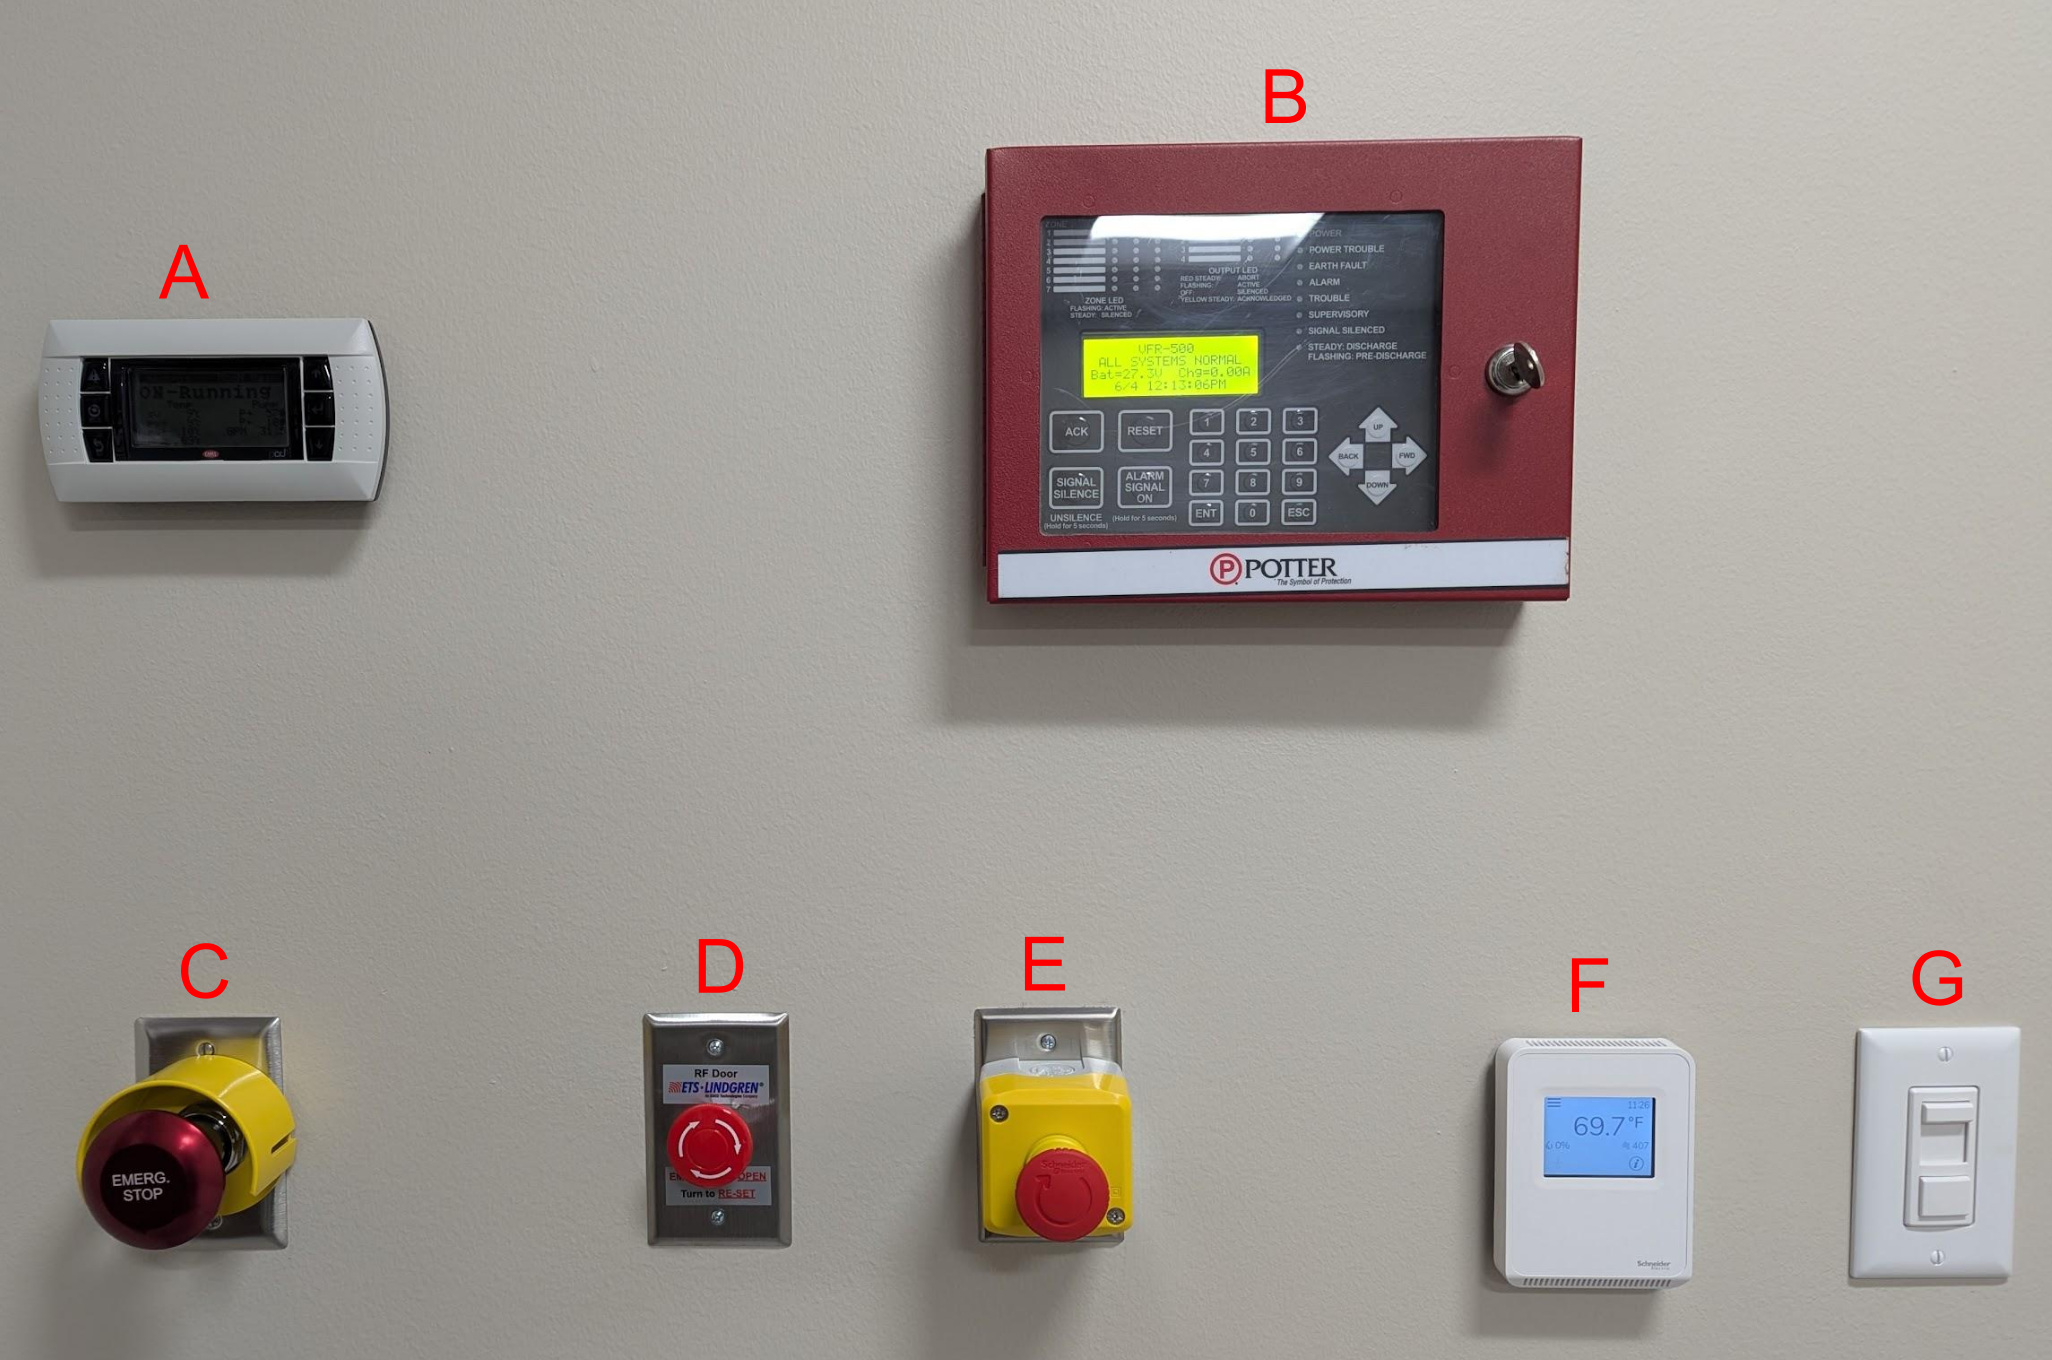
\includegraphics[width=0.95\textwidth]{button_wall.jpg}
	\caption{Control Room button wall. \textbf{A} Haskris Coolant Sounder. \textbf{B} Fire System Board. \textbf{C} Emergency Power Off. \textbf{D} Magnet Door release. \textbf{E} Unknown (potentially electric power off). \textbf{F} Thermostat. \textbf{G} Light switch.}
	\label{fig:button-wall-con}
\end{figure}

% Zone 3 fire ext
\begin{figure}[H]
	\centering
	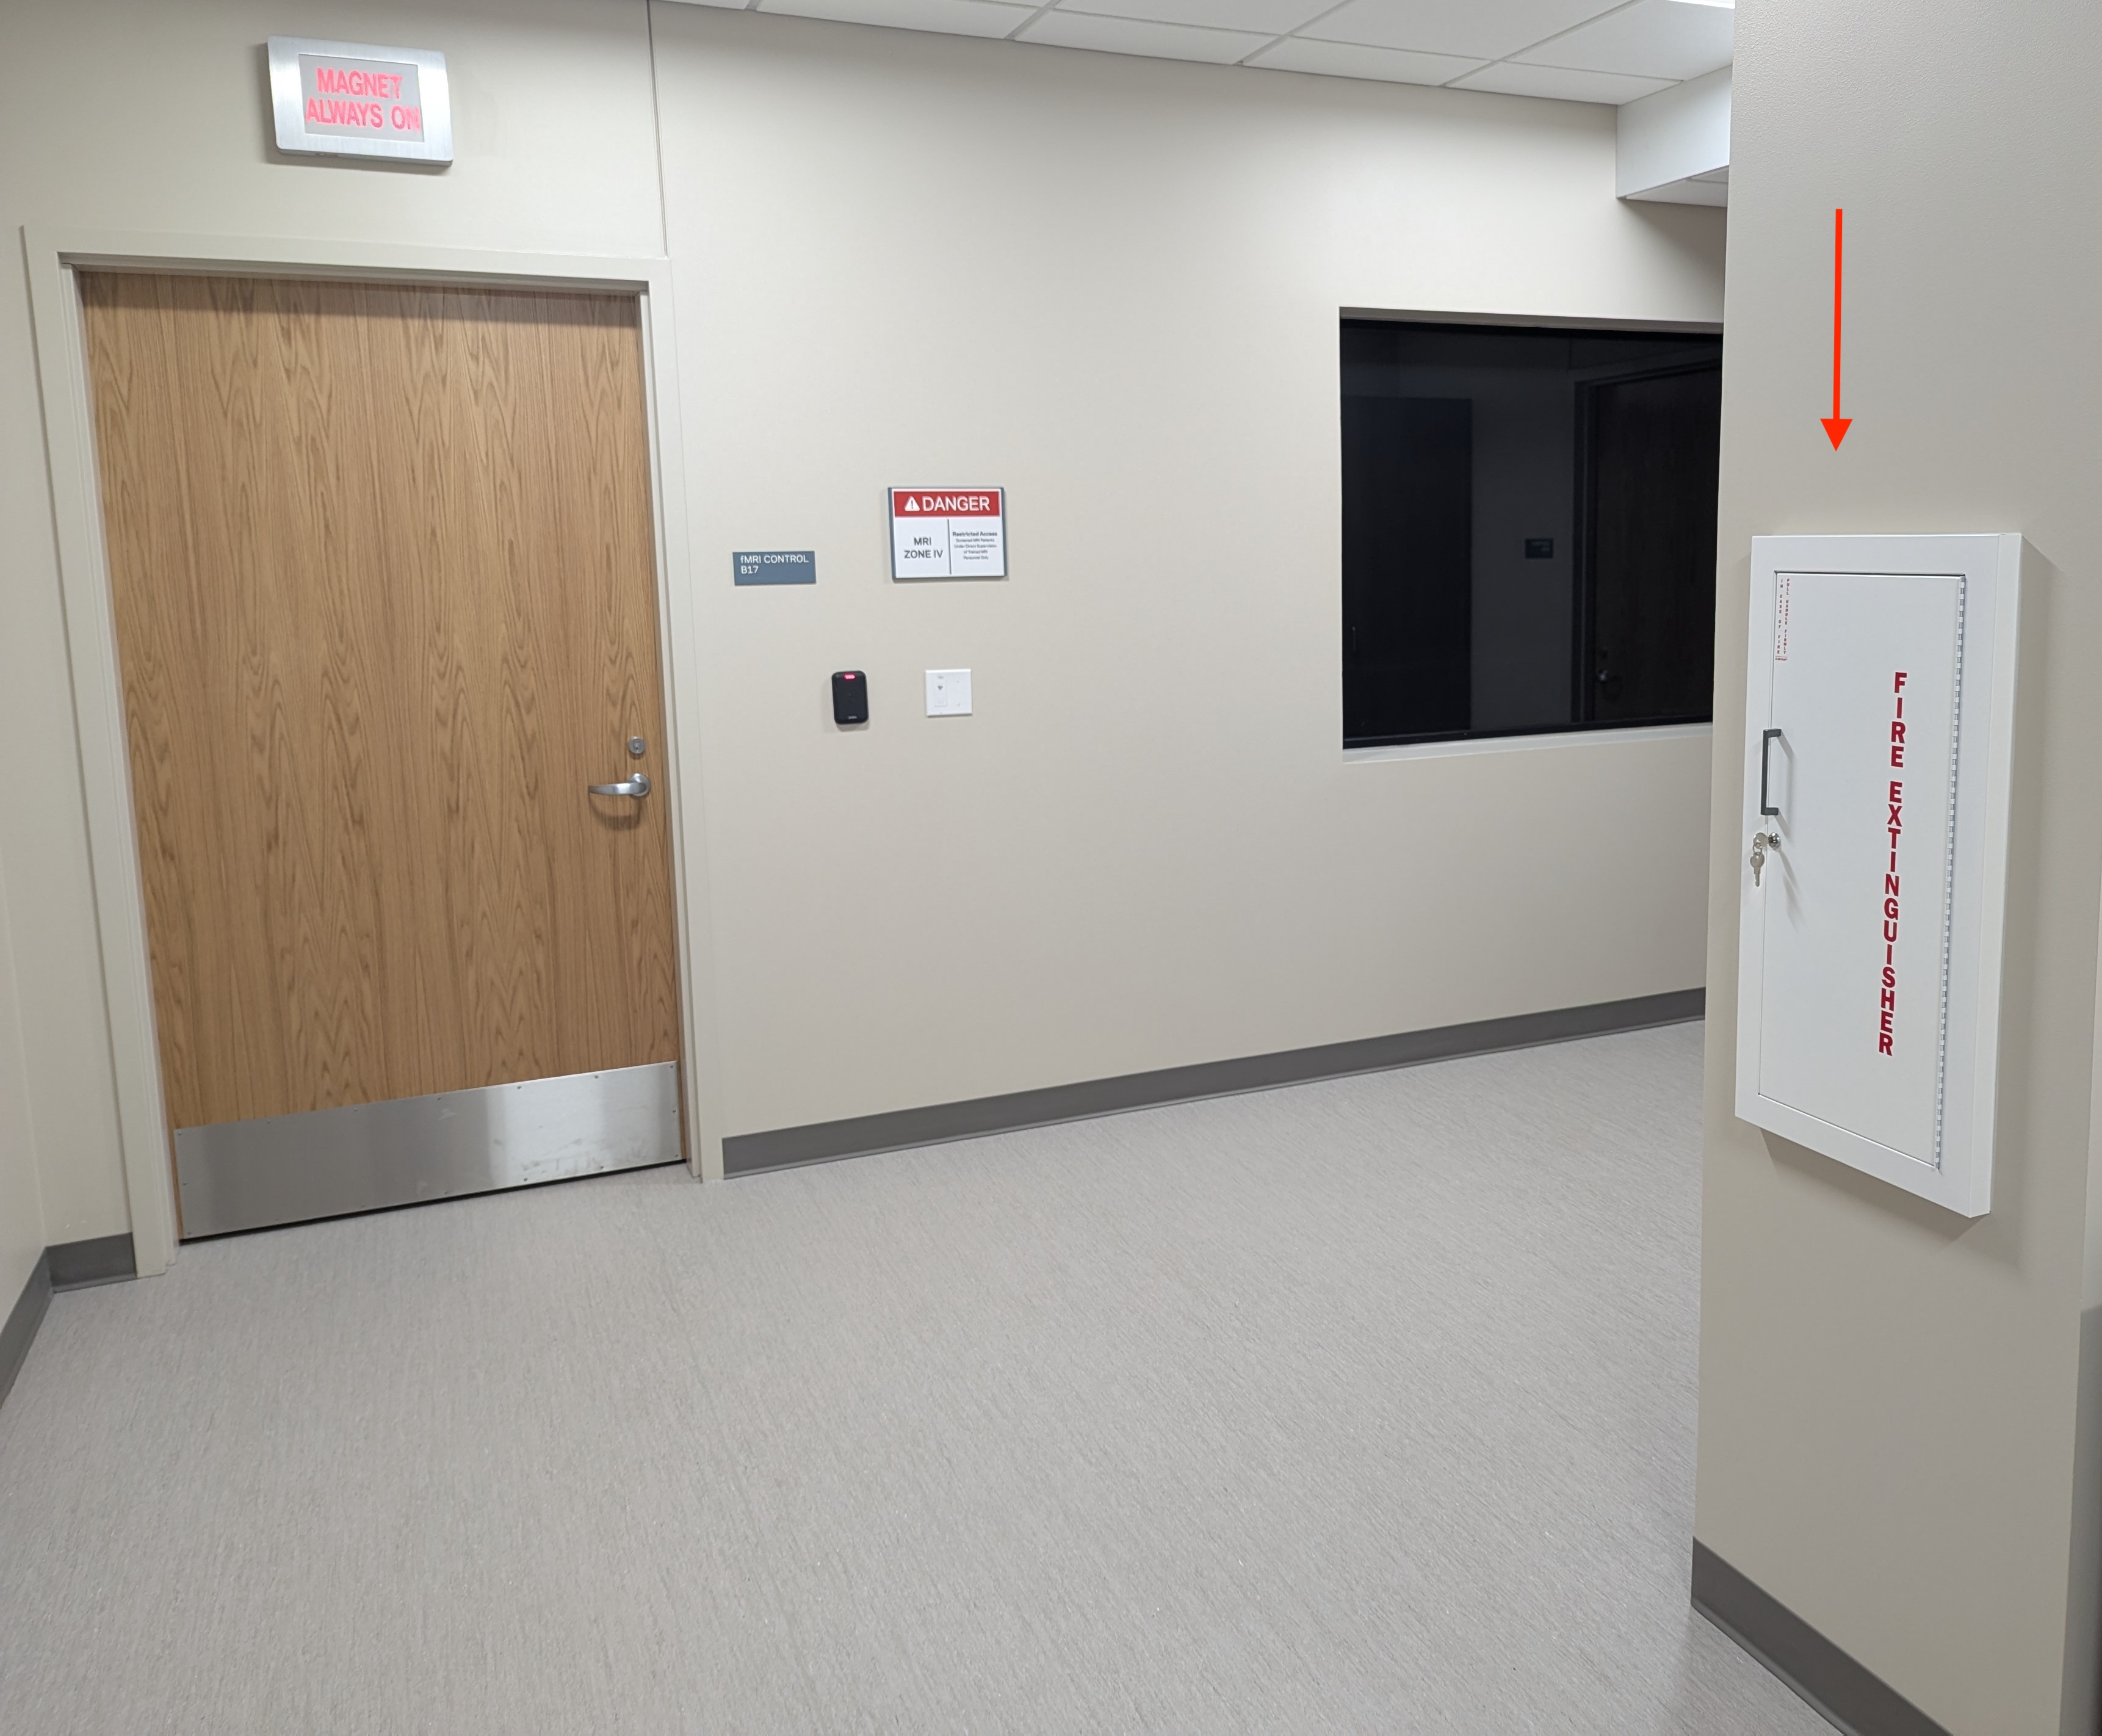
\includegraphics[width=0.95\textwidth]{fire_extinguisher_zone3.jpg}
	\caption{Zone 3 (B15) fire extinguisher (red arrow).}
	\label{fig:fire-ext}
\end{figure}

% Fire alarm
\begin{figure}[H]
	\centering
	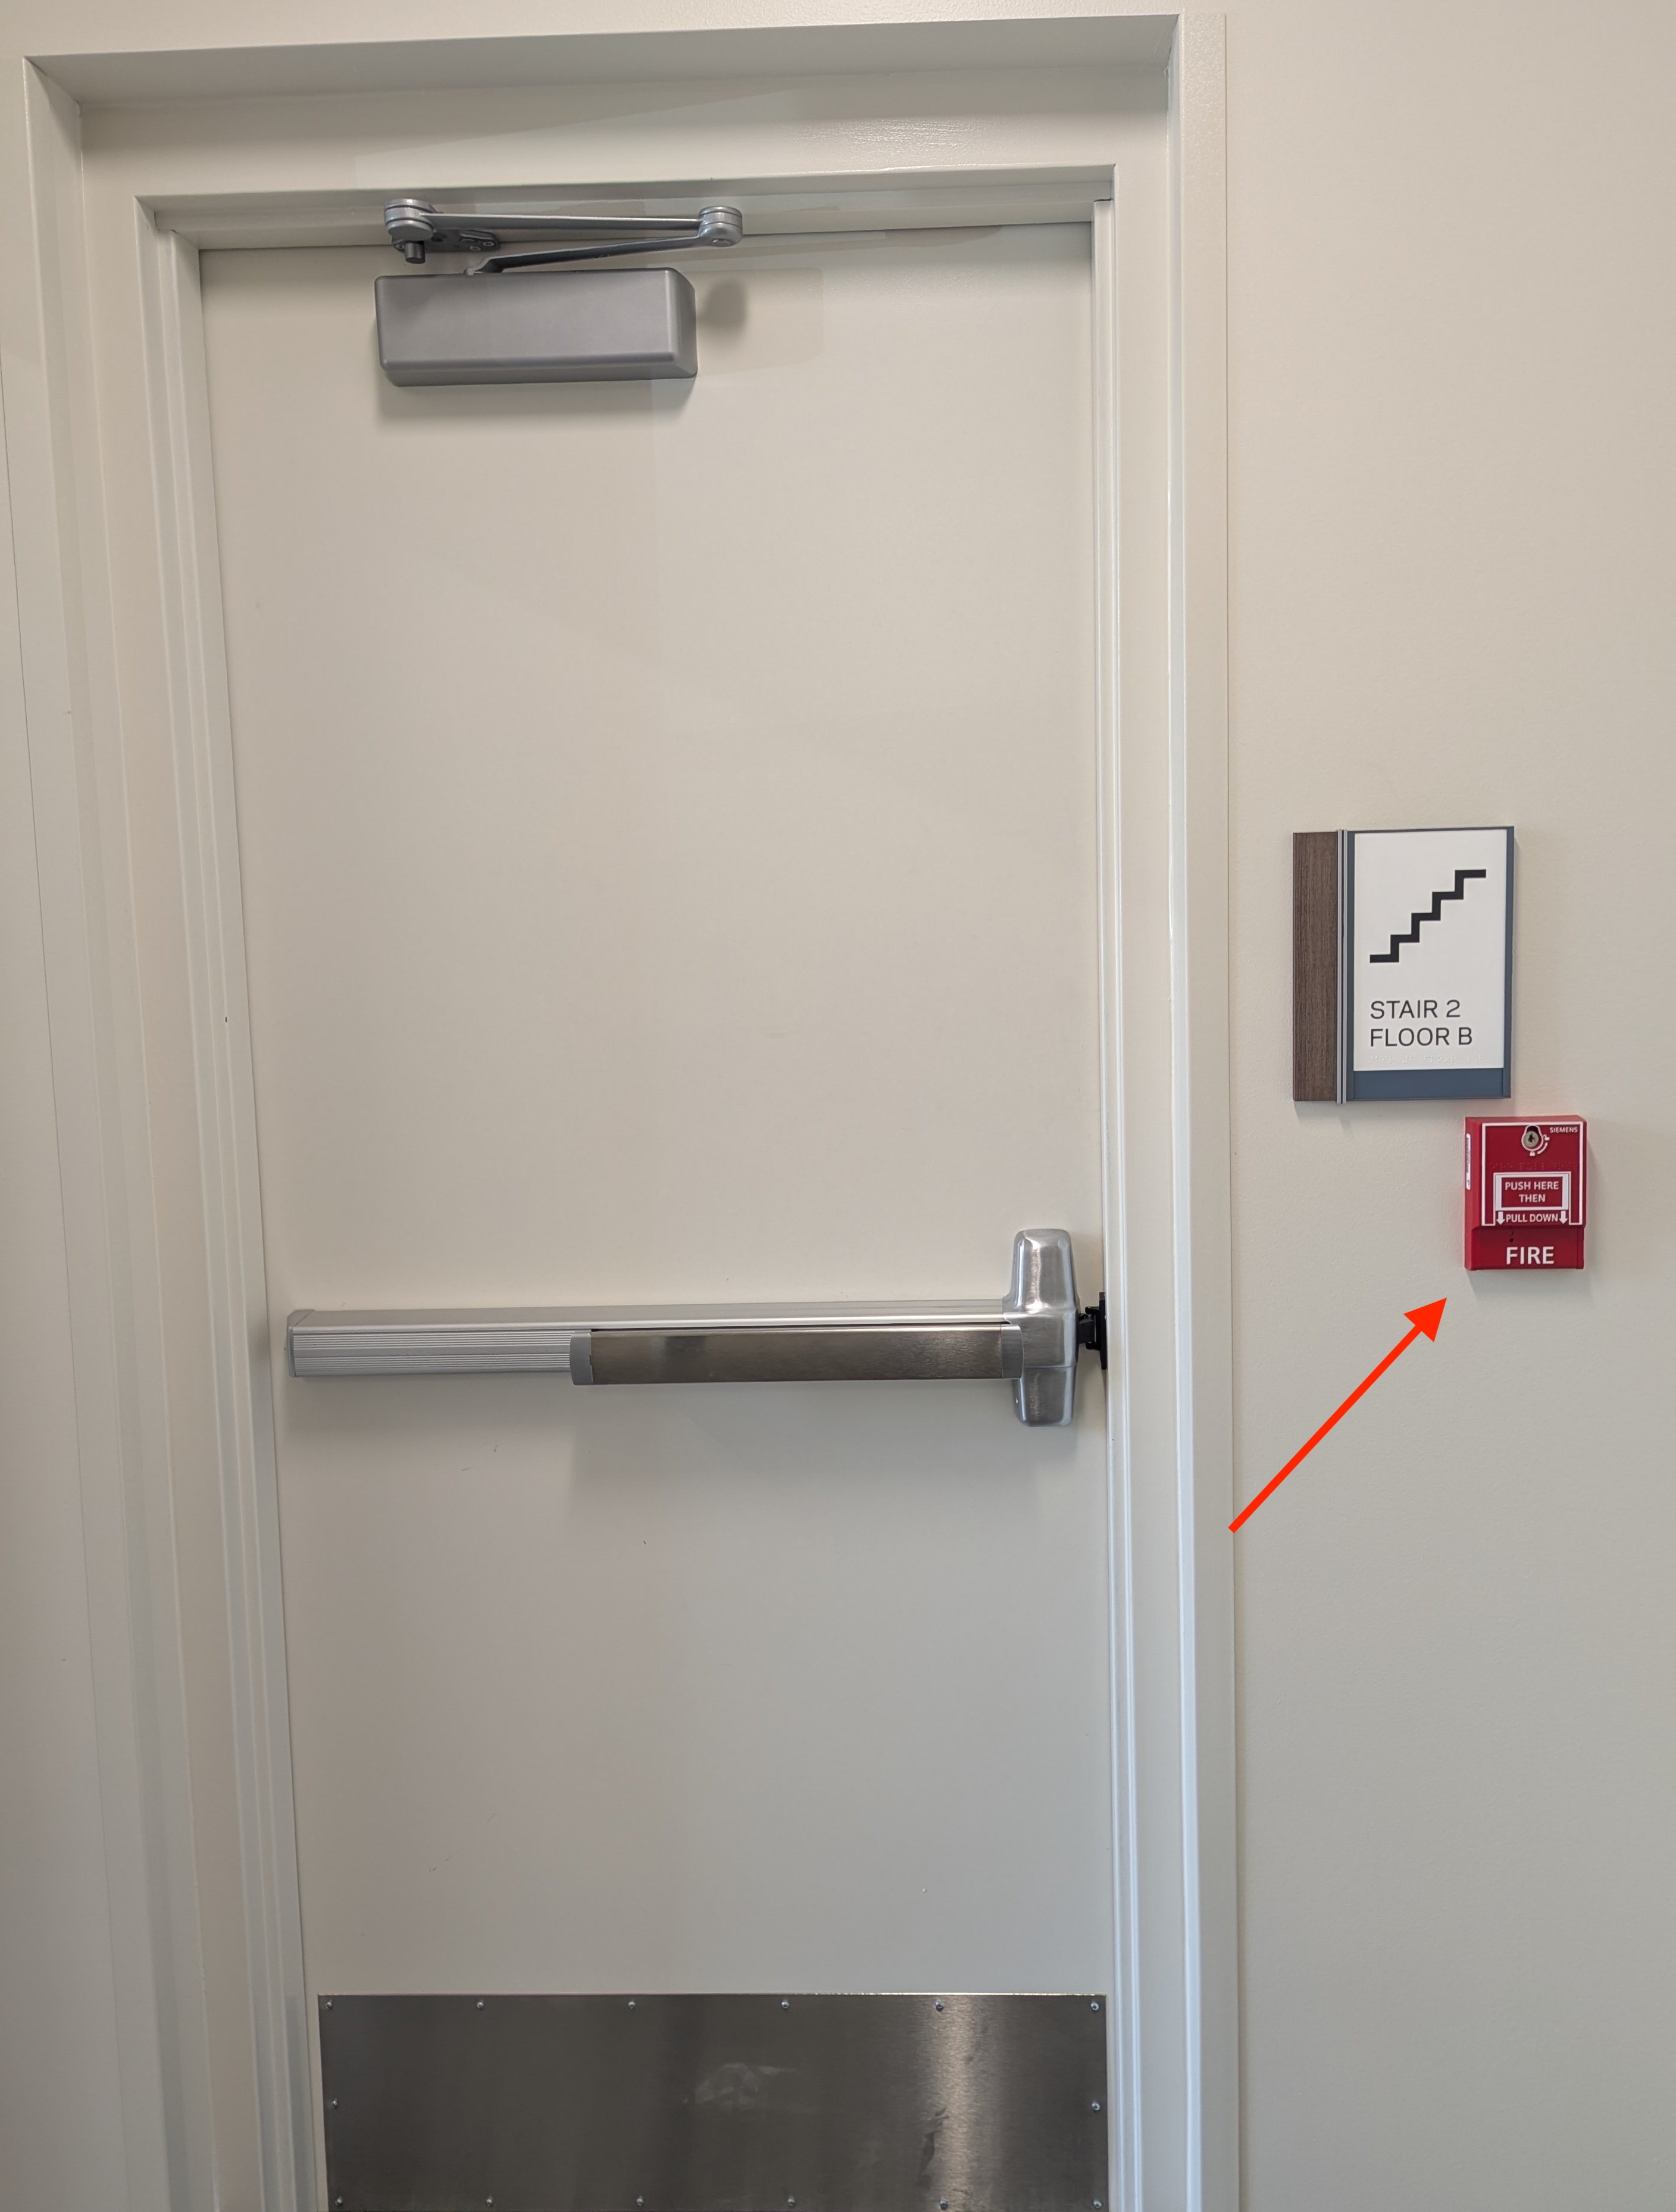
\includegraphics[width=0.95\textwidth]{fire_alarm.jpg}
	\caption{Lower level fire alarm, south door (red arrow).}
	\label{fig:fire-alarm}
\end{figure}

% Oxygen
\begin{figure}[H]
	\centering
	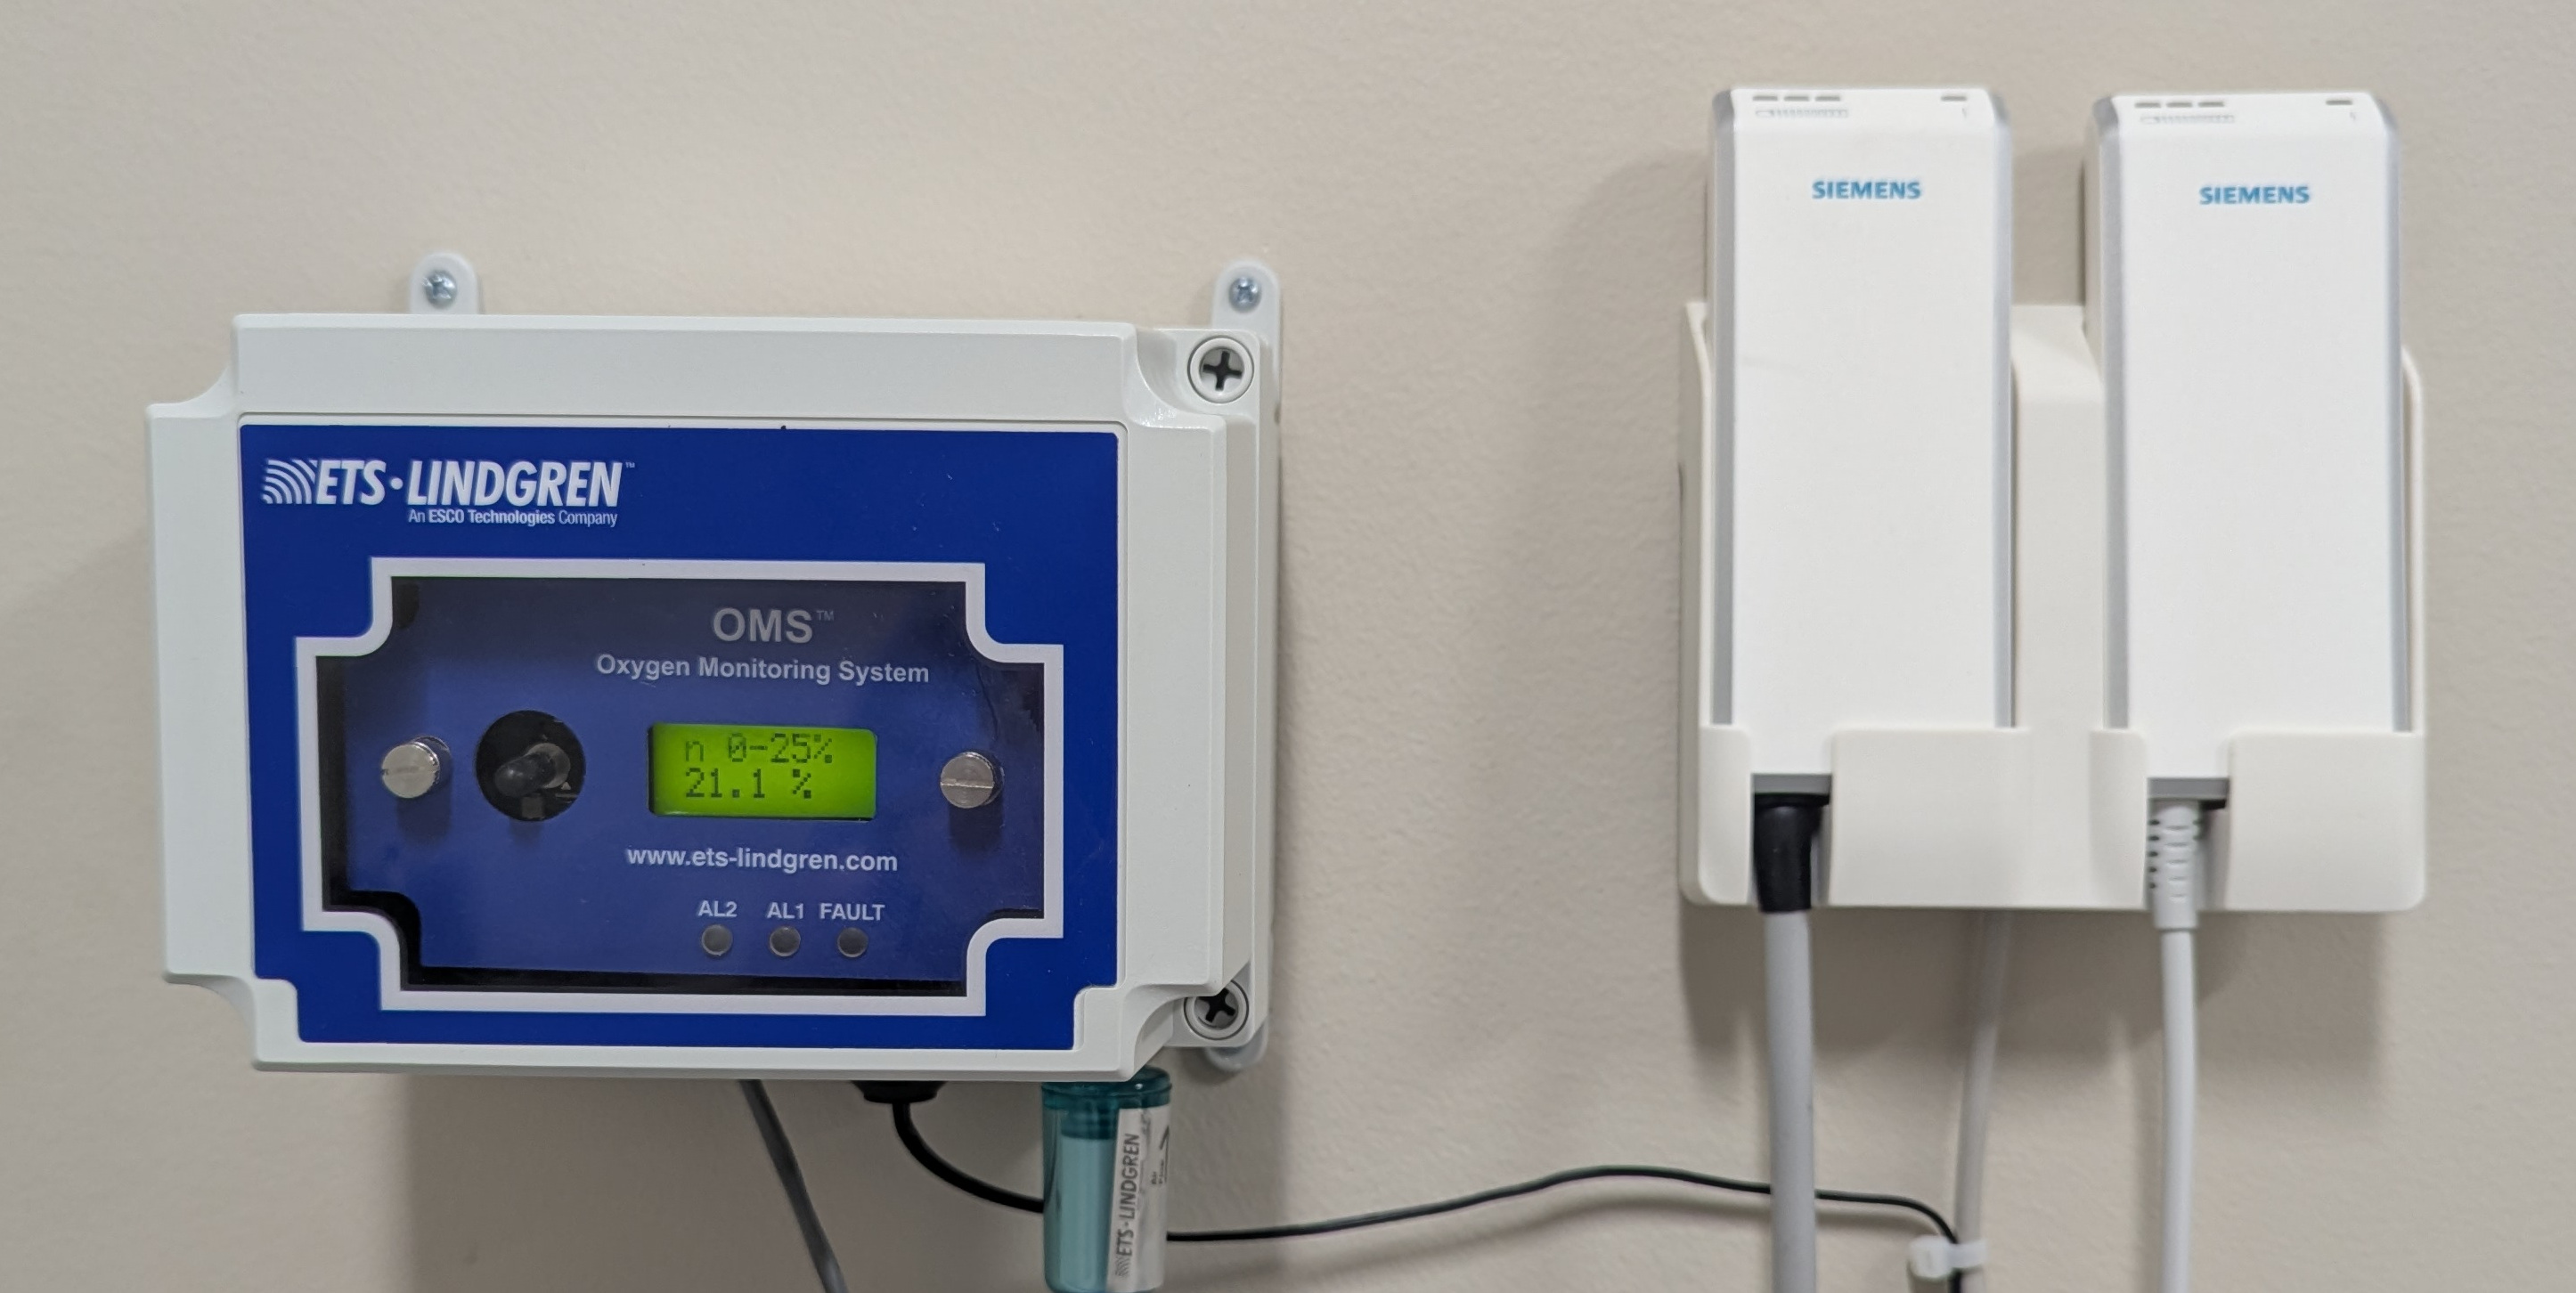
\includegraphics[width=0.95\textwidth]{oxygen_sensor.jpg}
	\caption{Control Room oxygen sensor (left) and psychopysiologic equipment (right).}
	\label{fig:oxygen}
\end{figure}

% Alarms
\begin{figure}[H]
	\centering
	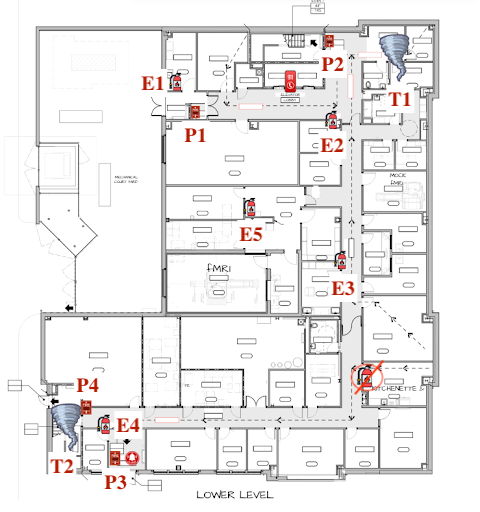
\includegraphics[width=0.7\textwidth]{vfpc_floor0.png}
	\caption{ND-HNC location of fire extinguishers (E1-5), alarm pulls (P1-4), and tornado shelters (T1-2). Crossed extinguisher indicates extinguisher does not exist in location.}
	\label{fig:vfpc-floor0}
\end{figure}

% Rendezvous location
\begin{figure}[H]
	\centering
	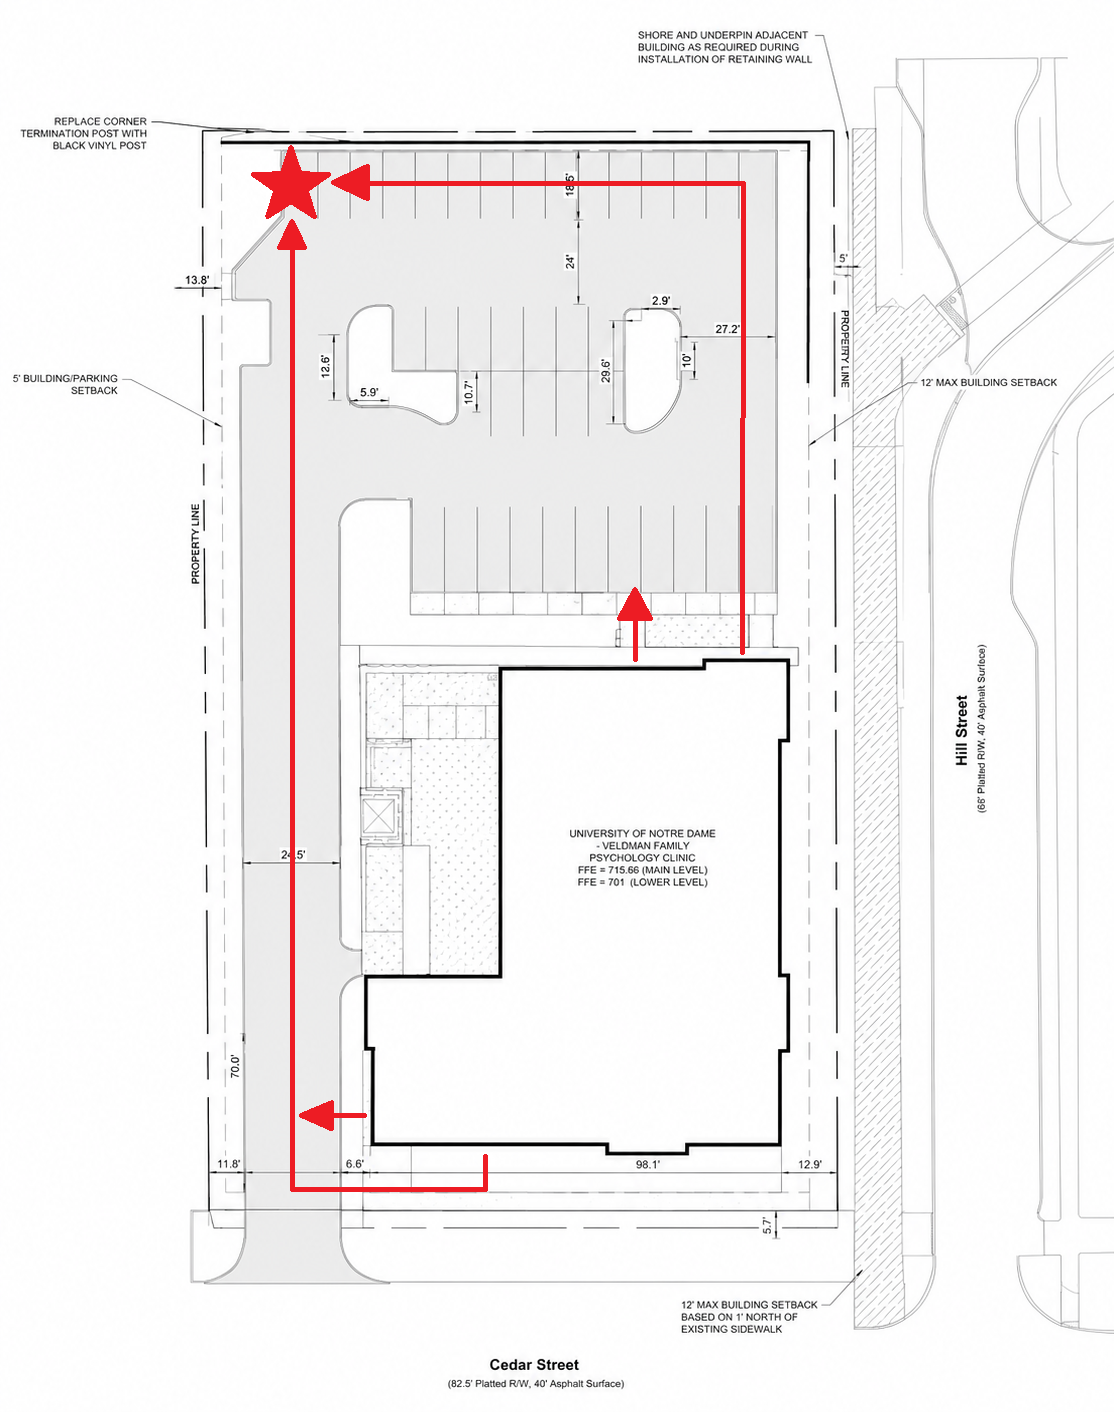
\includegraphics[width=\textwidth]{vfpc_rendezvous.png}
	\caption{VFPC rendezvous location.}
	\label{fig:vfpc-rend}
\end{figure}

% Power switch
\begin{figure}[H]
	\centering
	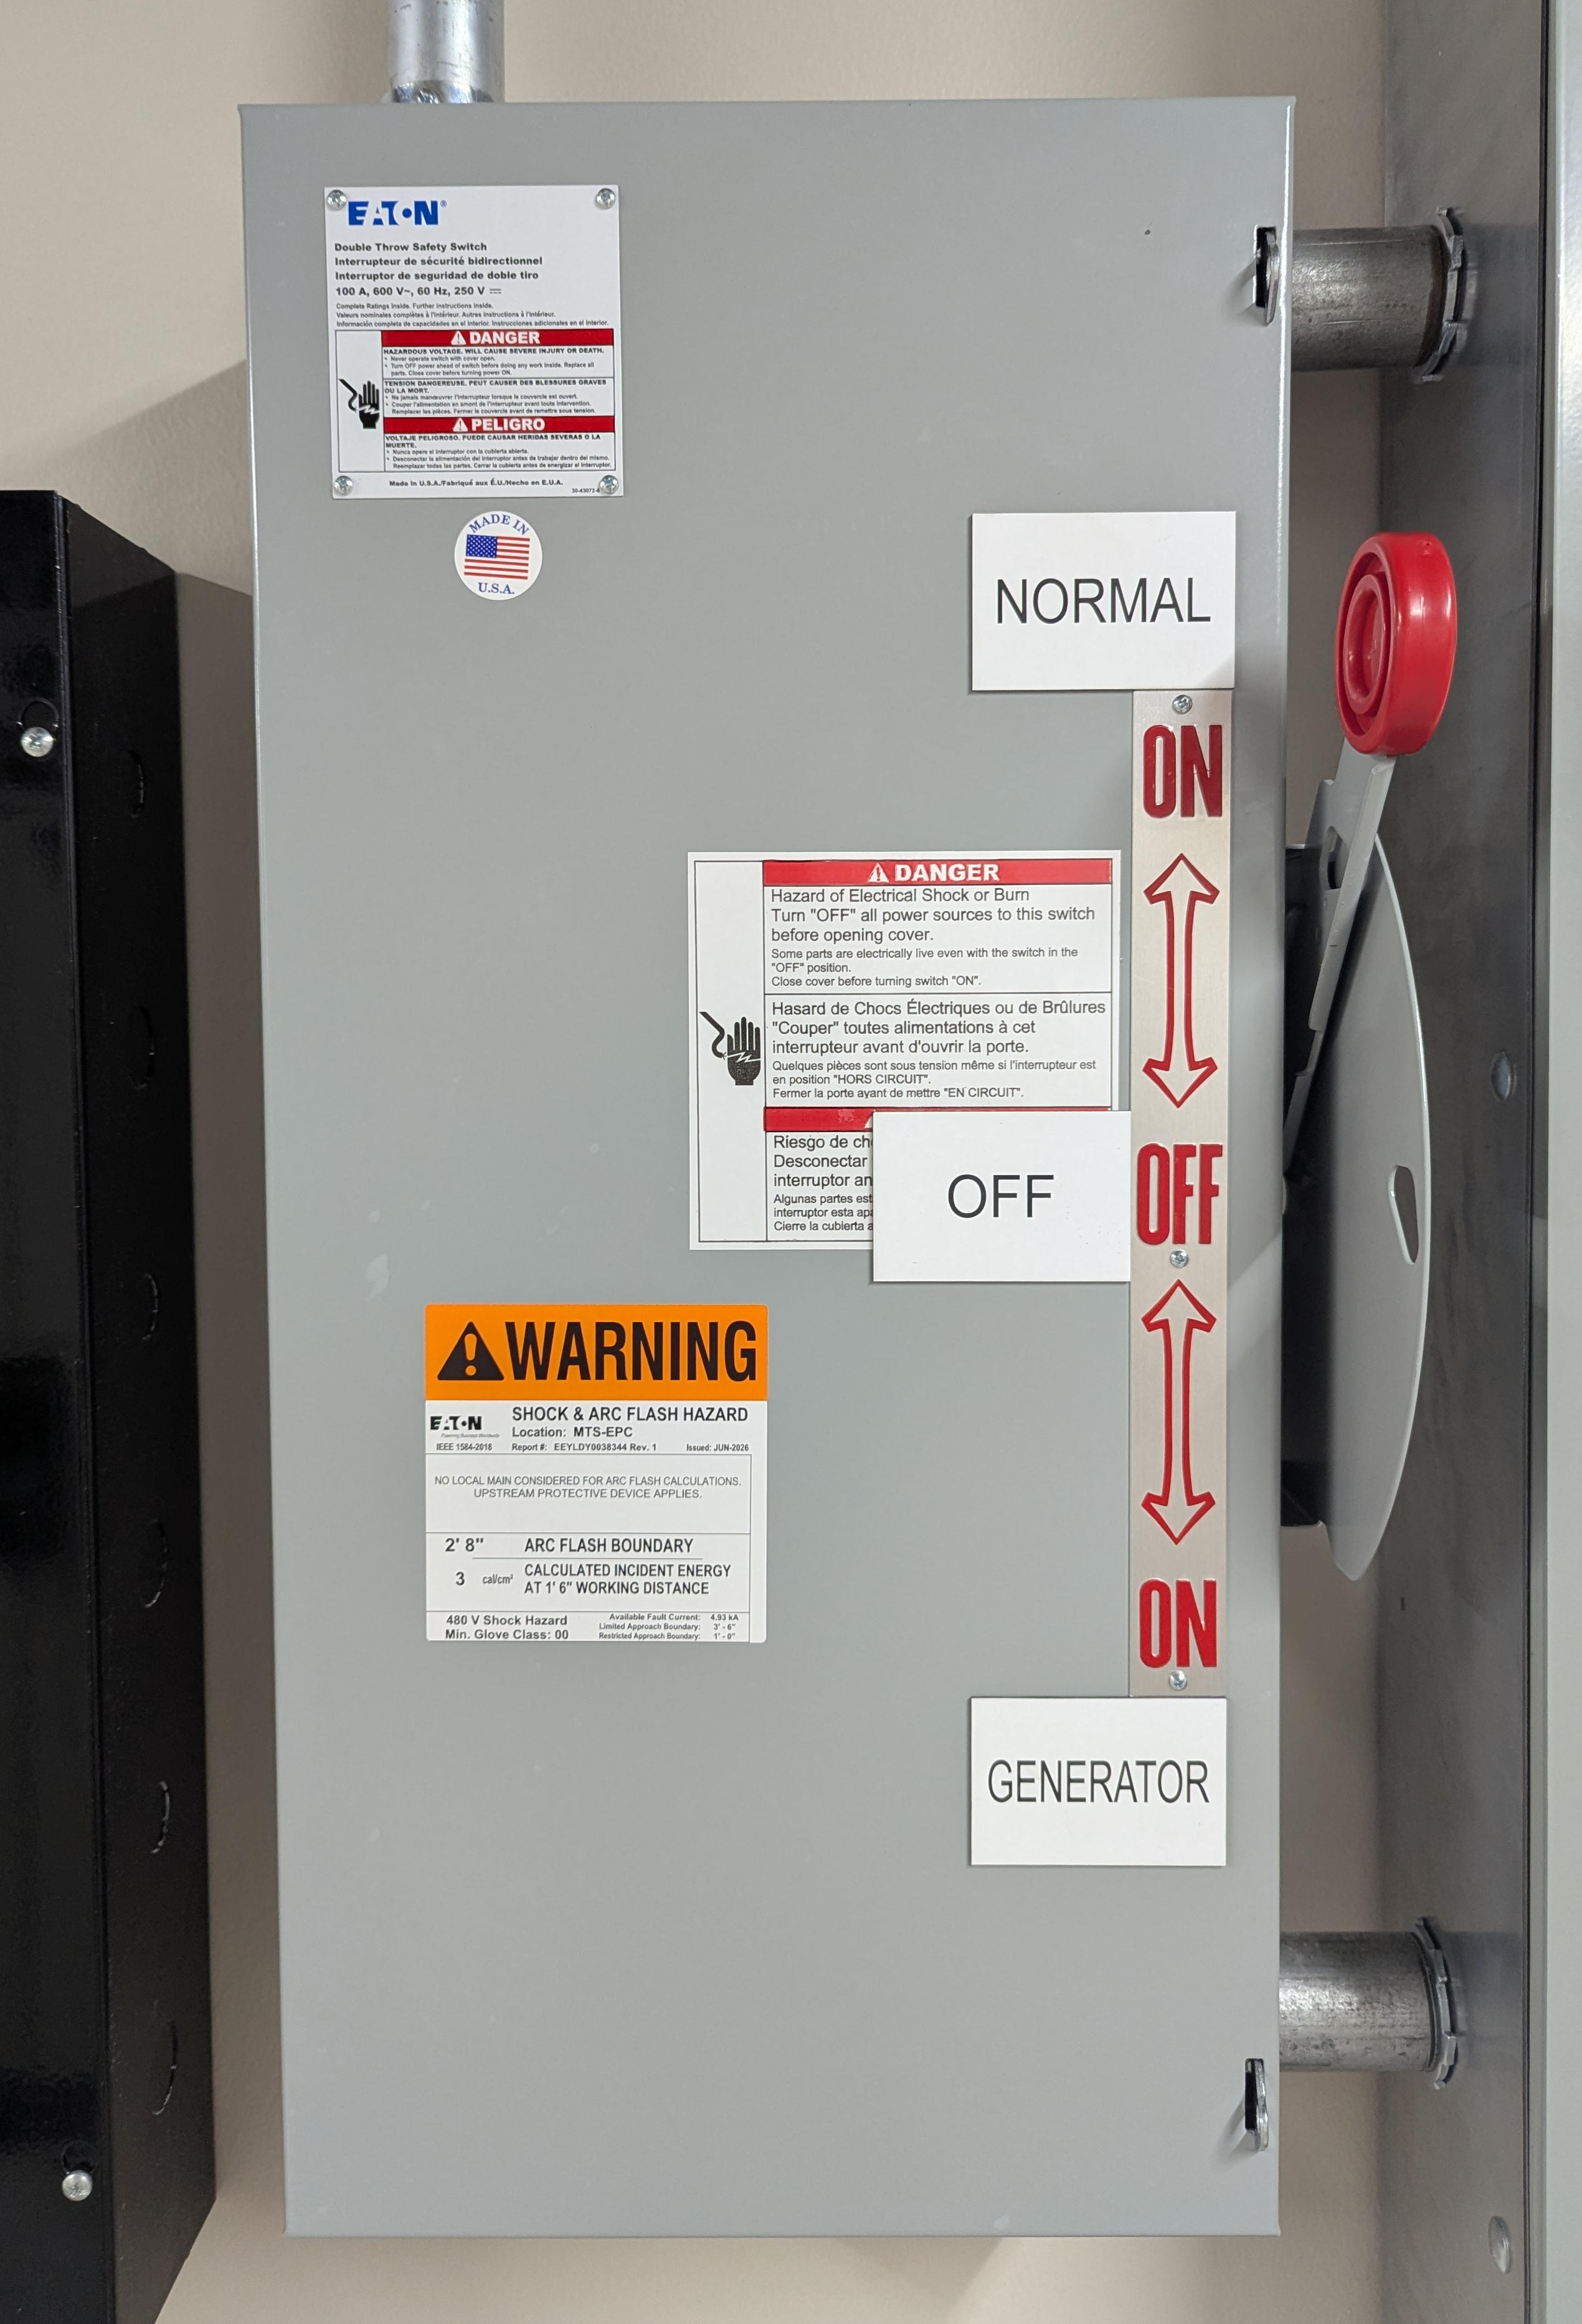
\includegraphics[width=0.7\textwidth]{switch_generator.jpg}
	\caption{Cooling pump power switch.}
	\label{fig:power-switch}
\end{figure}


\end{document}